% $Id: INF_Poster.tex 7714 2011-08-31 17:34:46Z tkren $
%
% TU Wien - Faculty of Informatics
% poster template
%
% This template is using the beamer document class and beamerposter package, see
% <http://www.ctan.org/tex-archive/macros/latex/contrib/beamer/>
% <http://www.ctan.org/tex-archive/macros/latex/contrib/beamerposter/>
% <http://www-i6.informatik.rwth-aachen.de/~dreuw/latexbeamerposter.php>
%
% For questions and comments send an email to
% Thomas Krennwallner <tkren@kr.tuwien.ac.at>
%

\documentclass[final,hyperref={pdfpagelabels=true}]{beamer}

\usepackage{TUINFPST}
\usepackage{lipsum}

\title[Software Engineering \& Internet Computing]{Simulation of different selfish mining strategies in Bitcoin}
% if you have a long title looking squeezed on the poster, just force
% some distance:
% \title[Computational Intelligence]{%
%   Integration of Conjunctive Queries over \\[0.2\baselineskip]%
%   Description Logics into HEX-Programs %\\[0.2\baselineskip]%
% }
\author[simon.mulser@gmail.com]{Simon Mulser}
\institute[]{%
  Technische Universit{\"a}t Wien\\[0.25\baselineskip]
  Institut f{\"u}r Information Systems Engineering\\[0.25\baselineskip]
  Arbeitsbereich: Information \& Software Engineering\\[0.25\baselineskip]
  BetreuerIn: Privatdoz. Mag.rer.soc.oec. Dipl.-Ing. Dr.techn. Edgar Weippl
}
\titlegraphic{
\includegraphics[height=52mm]{ifs_logo}}
\date[\today]{\today}
\subject{epilog}
\keywords{my kwd1, my kwd2}

%%%%%%%%%%%%%%%%%%%%%%%%%%%%%%%%%%%%%%%%%%%%%%%%%%%%%%%%%%%%%%%%%%%%%%%%%%%%%%%%%%%%%%

% Display a grid to help align images 
%\beamertemplategridbackground[12.7mm]

% play around with the background colors
% \setbeamercolor{background canvas}{bg=yellow}

% use a background picture
% \usebackgroundtemplate{%
%   
\includegraphics[width=\paperwidth]{logo_KBS_2_CMYK}
% }

% play around with block colors
\setbeamercolor{block body}{fg=black,bg=white}
\setbeamercolor{block title}{fg=TuWienBlue,bg=white}
\setbeamertemplate{caption}{\raggedright\insertcaption\par}

\setbeamertemplate{block begin}{
  \begin{beamercolorbox}{block title}%
    \begin{tikzpicture}%
      \node[draw,rectangle,line width=3pt,rounded corners=0pt,inner sep=0pt]{%
        \begin{minipage}[c][2cm]{\linewidth}
          \centering\textbf{\insertblocktitle}
        \end{minipage}
      };
    \end{tikzpicture}%
  \end{beamercolorbox}
  \vspace*{1cm}
  \begin{beamercolorbox}{block body}%
}

\setbeamertemplate{block end}{
  \end{beamercolorbox}
  \vspace{2cm}
}

% setup postit
\setbeamercolor{postit}{fg=black,bg=yellow} 
\newenvironment{postit}
{\begin{beamercolorbox}[sep=1em,wd=7cm]{postit}}
{\end{beamercolorbox}}


% for crop marks, uncomment the following line
\usepackage[cross,width=88truecm,height=123truecm,center]{crop}

%%%%%%%%%%%%%%%%%%%%%%%%%%%%%%%%%%%%%%%%%%%%%%%%%%%%%%%%%%%%%%%%%%%%%%%%%%%%%%%%%%%%%%

\begin{document}

% We have a single poster frame.
\begin{frame}
  \begin{columns}[t]

    \begin{column}{.35\textwidth}
      \begin{block}{Context}
      	Selfish mining is an attack on the Bitcoin mining process.
      	Recent research showed that the selfish miner can increase the relative gain on mining rewards compared to the rest of the network.
      	The miner achieves this by withholding found blocks, which it then later uses to match or overwrite blocks found by the honest miners.
      	The attack comprises the idea that the miner lets the rest of the network waste their computational power on mining blocks which do not end up in the longest chain.
      \end{block}
      
    \end{column}

    \begin{column}{.55\textwidth}
    
      \begin{block}{Goals}
      Development of a novel, more accurate simulation framework which:
      	\begin{itemize}
      		\item naturally respects the the peer-to-peer network and its latency
      		\item directly reuses the reference implementation to capture all protocol details and to avoid time-consuming and error-prone adaptation or abstraction of the protocol
      	\end{itemize}
      Afterwards:
         \begin{itemize}
         	\item Implement selfish mining strategies in a proxy which eclipses a normal node
      		\item Simulate different selfish mining strategies under a realistic scenario
      		\item Determine best performing strategies and compare them with honest mining
      		\item Contrast the obtained results with simulations of previous research
      	\end{itemize}
      \end{block}
    \end{column}

  \end{columns}

  \begin{block}{Simulation Framework}
  \begin{columns}[t]

    \begin{column}{.3\textwidth}
		
		\begin{figure}[t]
		    \vspace*{-1cm}
			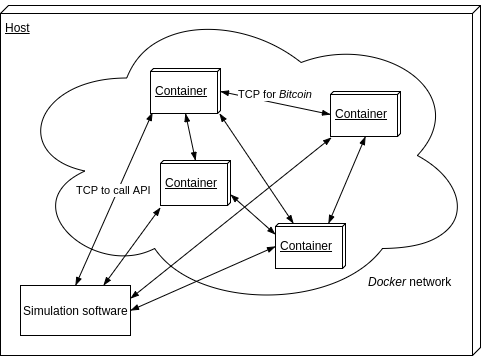
\includegraphics[width=20cm]{overview_setup}
			\centering
			\caption{Virtual peer-to-peer network with \textit{Docker}}
		\end{figure}      	
      
    \end{column}

    \begin{column}{.6\textwidth}
    	Network:
     	\begin{itemize}
     		\item \textit{Docker} is used to virtualise the whole peer-to-peer network
     		\item Latency is applied to the TCP-connections between the nodes by using \textit{Unix tc}
     		\item In the \textit{Docker} container the actual Bitcoin reference implementation is executed
     		\item Bitcoin nodes are not mining but are creating blocks on RPC-call from framework
     	\end{itemize}
     	Simulation:
       	\begin{itemize}
     		\item Network is set-up by framework based on pre-defined scenario
     		\item Nodes generate blocks based on samples drawn from an exponential distribution
     		\item Safety checks if simulation is executed to fast by splitting real time into multiple spans
     		\item After a simulation run log-files of nodes are parsed and calculated statistics are summarised in report 	\end{itemize}
    \end{column}

  \end{columns}
  \end{block}
  
  \begin{block}{Selfish Proxy}
  	\begin{columns}[t]
     	\begin{column}{.45\textwidth}
     		Node in the network which eclipses a normal Bitcoin node from the rest of the network. By withholding blocks from the eclipsed node to the honest network and vice versa, the selfish proxy is able to mimic different selfish mining strategies.
     		
     		\bigskip
     		Advantages:
     		\begin{itemize}
     			\item No need to alter Bitcoin reference implementation
     			\item Possibility to extend node for other attacks
			\end{itemize}
     		Disadvantage:
     		\begin{itemize}
     			\item Part of the Bitcoin protocol and the current state of the blockchain needs to be handled
     			\item Introduces extra hop and thus, impacts performance of selfish mining algorithms
			\end{itemize}   			
    	\end{column}
 	
        \begin{column}{.45\textwidth}
        	\begin{figure}[t]
        	    \vspace*{-1cm}
            	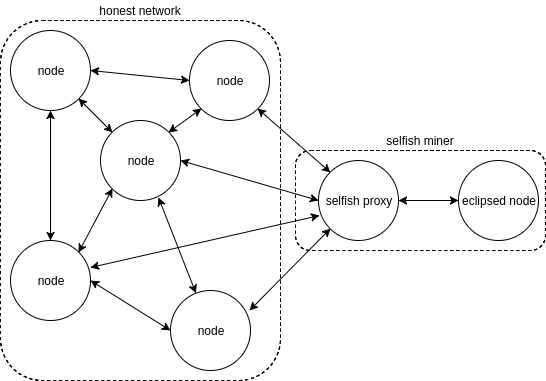
\includegraphics[width=23cm]{selfish_proxy}
            	\centering
            	\caption{Selfish proxy eclipsed node to perform selfish mining}
        	\end{figure} 
    	\end{column}
    	
  	\end{columns}
  \end{block}

  \begin{columns}[t]

    \begin{column}{.55\textwidth}
      \begin{block}{Results}
		
		\begin{columns}[t]

    		\begin{column}{.45\textwidth}
        		\begin{figure}[t]
        			\vspace*{-1cm}
            		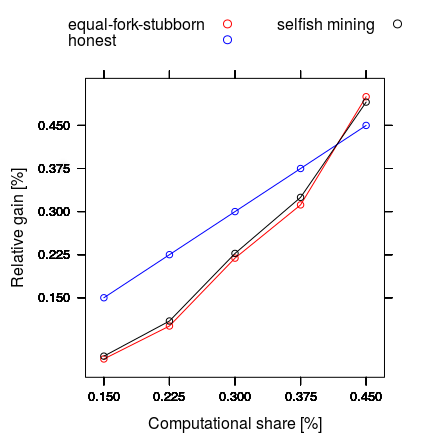
\includegraphics[width=18cm]{relative_block_share}
            		\centering
            		\caption{Relative gain of different mining methods}
        		\end{figure}
    		\end{column}
    		\begin{column}{.45\textwidth}
				\begin{itemize}
					\item Simulation showed that selfish mining increases the relative gain compare to honest mining
					\item With a computation power of 45\% the selfish miner can gather about 50\% of the mining rewards
					\item Best performing strategies are equal-fork-stubborn and selfish mining
				\end{itemize}
    		\end{column}
  		\end{columns}
  		
      \end{block}  
                
    \end{column}

    \begin{column}{.35\textwidth}
    
      \begin{block}{Additional Outcome}
      	\begin{itemize}
     		\item RQ1: Do the simulations of selfish mining with the proposed software solutions
show an increase of the total and relative gain for the selfish miner compared to
the normal, honest mining behaviour?
			\item RQ2: How do the obtained results of the simulation match the outcome of previous
research in the area of selfish mining?
      	\end{itemize}
      \end{block}

    \end{column}

  \end{columns}

\end{frame}

\end{document}

%%% Local Variables:
%%% TeX-PDF-mode: t
%%% TeX-debug-bad-boxes: t
%%% TeX-master: t
%%% TeX-parse-self: t
%%% TeX-auto-save: t
%%% reftex-plug-into-AUCTeX: t
%%% End:
